\documentclass[10pt]{beamer}

\usetheme[progressbar=frametitle]{metropolis}
\usepackage{appendixnumberbeamer}

\usepackage{booktabs}
\usepackage[scale=2]{ccicons}

\usepackage{pgfplots}
\usepgfplotslibrary{dateplot}

\usepackage{xspace}
\newcommand{\themename}{\textbf{\textsc{metropolis}}\xspace}

\usepackage{graphicx}
\graphicspath{ {./images/} }



\title{Adversarial Deep Learning Models with Multiple Adversaries Presentation}
\subtitle{A Presentation}
\author{Khan Saad Bin Hasan \newline 16PEB121 \newline GH3571}
\institute{Zakir Husain College Of Engineering and Technology \newline Aligarh Muslim University, Aligarh}
\date{\today}


\begin{document}

\maketitle

\begin{frame}{Table of contents}
  \setbeamertemplate{section in toc}[sections numbered]
  \tableofcontents%[hideallsubsections]
\end{frame}

\section[Introduction]{Introduction}

\begin{frame}[fragile]{Paper in a Nutshell}
    \begin{itemize}
    		\item We make an adversary and a player, they play against each other. The adversary generates data that can attack the model and produce such examples that will generate false results from the model. For example, Negative results appear positive. 
    		\item This can be a security flaw, hence to make the model robust against such attacks we generate this data ourselves by attacking the model and collecting the data.
    		\item This data is then used to retrain the model and hence after retraining the model is more secure toward such attacks.
    		\item Our adversarial algorithm proposes a game between two players—a data miner or learner and an intelligent adversary or adversary. The interactions between the learner and adversary are modelled as a two-player sequential Stackelberg zero-sum game. In our game, the adversary is the leader and the learner is the follower. The learner retrains the model after the adversary’s attack. 
    \end{itemize}
\end{frame}

\section[Tools, Techniques and Algorithms used]{Tools, Techniques and Algorithms used}

\subsection{Adversarial Learning}

\begin{frame}{Tools, Techniques and Algorithms used- Adversarial Learning}
	\begin{itemize}
		\item {\bf Adversarial learning} algorithms are specifically designed to exploit vulnerabilities in a given machine learning algorithm. 
		\item These vulnerabilities are simulated by training the learning algorithm under various attack scenarios and policies. The attack scenarios are assumed to be formulated by an intelligent adversary.
		\item A learning algorithm designed over adversarial settings becomes robust to such vulnerabilities in the training and testing data distributions.
		\item In high dimensional data, deep learning has been found to be susceptible to adversarial examples \cite{goodfellow2014generative}. 
	\end{itemize}
\end{frame}


\subsection{Game Theory}

\begin{frame}{Tools, Techniques and Algorithms used- Game Theory}
	\begin{itemize}
		\item {\bf Game Theory} is the study of interactions or games between independent self-interested agents or players. 
		\item Each player has a set of associated strategies/moves/actions that optimize a payoff function or utility function. 
		\item The key idea in game theory is that of an equilibrium state from which none of the players have any incentive to deviate called {\bf Nash equilibrium}.
		\item A two-player game where a single follower acts in response to the moves of a single leader is called a {\bf Stackelberg game}.
	\end{itemize}
\end{frame}



\begin{frame}{Game-Theoretic Learning Models}
	\begin{itemize}
		\item The learner has no incentive to play a game that leads to too many false positives with too little increase in true positives.  
		\item The adversary has no incentive to play a game that increases the utility of false negatives not detected by the learning algorithm. 
		\item At equilibrium, the adversary is able to find testing data that is significantly different from the training data whereas the learner is able to update its model for new threats from adversarial data.
		\item The adversary iteratively attacks the data miner using the best possible strategy for transforming the original training data. The data miner independently reacts by rebuilding the classifier based on the data miner’s observations of the adversary’s modifications to the training data.
		\item The game is repeated until the adversary’s payoff does not increase or the maximum number of iterations is reached. 
	\end{itemize}
\end{frame}


\subsection{Genetic Algorithms}

\begin{frame}{Tools, Techniques and Algorithms used- Genetic Algorithm}
	\begin{itemize}
        \item Based on theory of biological evolution, Genetic Algorithms are modelled. We take a starting population, then let it evolve over time. We define how a fit population should look like. The algorithm should provide populations closer to the fit population as generations proceed.
        \item As input, the Algorithm requires the training data X train. Each example in the input data is a three dimensional tensor of RGB pixel values. 
        \item The standard {\bf selection, crossover, mutation, and clone} are used to generate population in the genetic algorithm.
	\end{itemize}
\end{frame}


\begin{frame}{Genetic Operators: Selection Function and Crossover Function}
	\begin{itemize}
        \item The {\bf selection operator} conducts a weighted sampling without replacement where the weights are proportional to the fitness function values for the current population. 
        \item The {\bf selection function} randomly samples the current population to return the selected candidates and the remaining candidates as the offspring and parents respectively.
        \item The {\bf crossover operation} is applied between the odd children and even children in the offspring. 
        \item The {\bf crossover function} randomly slices and swaps the pixels of the current children. The starting and ending indices for slicing are also selected randomly.
	\end{itemize}
\end{frame}


\begin{frame}{Genetic Operators: Mutation and Fitness function}
	\begin{itemize}
        \item Random mutations are applied to the pixels of each offspring. The {\bf mutation function} applies a mask of random integers that are added to the pixel values in the current child. 
        \item {\bf fitness function} calls an evaluation function to compute the performance metrics on the data subject to adversarial manipulation. These metrics are calculated subject to the current softmax probabilities of the learner.
	\end{itemize}
\end{frame}


\subsection{Simulated Annealing}

\begin{frame}{Tools, Techniques and Algorithms used- Simulated Annealing}
	\begin{itemize}
	    \item In metallurgy, as metal is heated and cooled again and again, it becomes stronger and more robust to external stress and forces applied among other benefits. We use this principle for a modified approach of hill climbing. In which we randomly move from one point to another based on a parameter called temperature. This prevents us from getting stuck in local minima.
        \item Within each iteration of the game, the candidate solutions are generated by the {\bf annealing operator}. For every temperature a number of candidate solutions are generated. 
        \item The masking process used in the operator allows for the randomized selection of tensor regions in the game’s search procedure. 
        \item The random masks are generated by the Boolean tensor mask and the sliced index mask alongwith the initialization mask passed as a function argument 
	\end{itemize}
\end{frame}


\begin{frame}{Simulated Annealing Algorithm}
	\begin{itemize}
        \item If a given candidate solution is found to be fitter than the best solution, then the best solution is updated.
        \item If an increase in adversary’s payoff is seen on the given candidate solution, then the adversarial manipulation is updated. 
        \item The corresponding fitness function values are also simultaneously updated. 
        \item The search procedure in simulated annealing is randomly restarted with a probability depending on the current fitness function and current temperature values. 
	\end{itemize}
\end{frame}


\section{Related Work}


\begin{frame}{Previous Work}
	\begin{itemize}
		\item Biggio et al. \cite{biggio2013security} discuss the learner’s defence mechanism in terms of an empirical framework extending the model selection and performance evaluation steps of pattern classification \cite{duda2012pattern}. 
		\item Goodfellow et al. \cite{goodfellow2014generative} argue for the need to have an adversarial training procedure with the objective to minimize the worst case error when the data is perturbed by an adversary. Goodfellow et al. \cite{goodfellow2014generative} propose a minmax game between two deep learning networks called Generative Adversarial Networks (GANs). 
		\item A variety of generative methods are available to create the perturbation between training and testing data distributions \cite{papernot2016towards}.
        \item Berthelot et al. \cite{berthelot2017began} propose BEGAN with a new loss function in the training algorithm. Chen et al. \cite{chen2016infogan} propose InfoGAN which uses generative learning models for unsupervised representation learning.
	\end{itemize} 
\end{frame}



\begin{frame}{Our Modified Approach to GAN}
	\begin{itemize}
		\item The objective of our research is to simulate a real adversarial attack scenario on two-label classification model in terms of cost to the adversary. 
		\item We seek to increase the classification performance when the data distribution is changed with a malicious intent. 
		\item Our objective function has cost and error terms defining the attack scenarios in adversarial data settings.
		\item In a minmax game formulation, we seek to create the datasets for attack scenarios in a discriminative learning model and supervised learning problem
		\item The generator is the leader of the game in minmax formulation for GAN, whereas in our minmax formulation an intelligent adversary leads the game. 

	\end{itemize}
\end{frame}





% \begin{frame}{Stochastic Optimization}
% 	\begin{itemize}
% 		\item The adversarial data samples are generated by the selection, crossover, mutation search operators in the genetic algorithm and the annealing search operator in the simulated annealing algorithm. 
% 		\item By using probabilistic hill climbing algorithms over Markov chains in multivariate models, the current search operators can be extended to defined explicit probabilistic distributions performing a complex neighbourhood search for the candidate solutions [29]. 
% 	\end{itemize}
% \end{frame}


\section{Game Formulation}

\begin{frame}{Sequential Game Formulation}
	\begin{itemize}
        \item A constant sum Stackelberg game is simulated between two players called Leader (L) and Follower (F). \item The leader initiates the game by making the first action/move/play. In our algorithm, the adversary is the leader and the learner is the follower. 
        \item We train a CNN as the learner. With knowledge of only the learner’s classification error, the adversary is assumed to target the true positives.
        \item In each iteration of the game, the learner trains the weights in the CNN layers for the input presented by the adversary. 
        \item The adversary then adapts the data manipulations to the weights trained by the CNN. Thus, each player’s move is based on the opponent’s last play.
	\end{itemize}
\end{frame}


\begin{frame}{Game Theoretic Learner Illustration}
	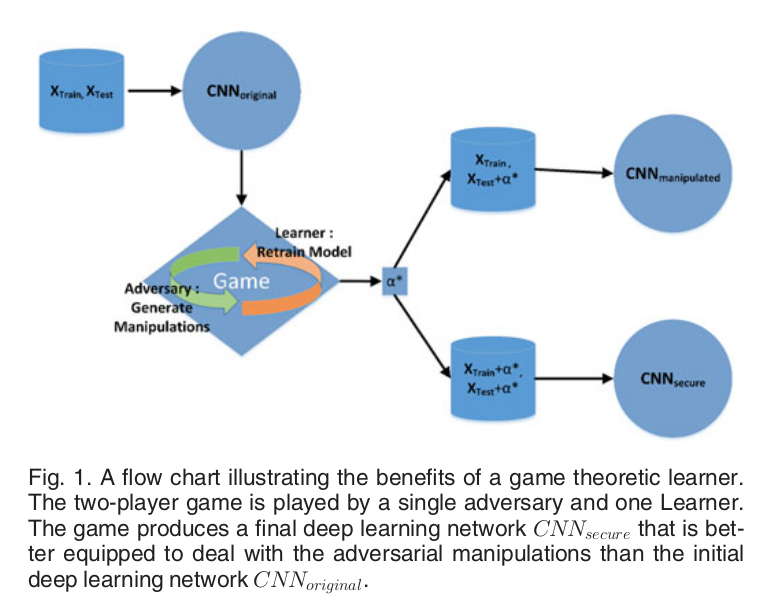
\includegraphics[scale=0.33]{images/Fig1}
\end{frame}


\begin{frame}{Examples Of Generated Data}
	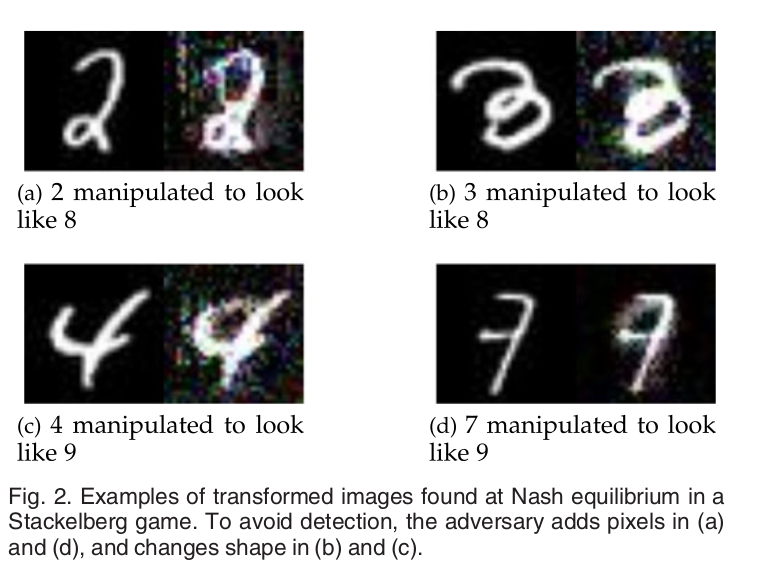
\includegraphics[scale=0.33]{images/Fig2}
\end{frame}


\begin{frame}{Stochastic Game Algorithm}
	\begin{itemize}
        \item As input, the algorithm requires the labelled training and testing data. 
        \item Each record in the training and testing data is a tensor with pixel values representing an image. 
        \item Initially the number of adversaries, is set to 1 for the two-player game. 
        \item The variable gametype allows each adversary in a multiplayer game to choose between Genetic Algorithm and Simulated Annealing as the optimization procedure for a two-player game.
	\end{itemize}
\end{frame}


\section{Experiments and Observations}

\begin{frame}{Experiments}
	\begin{itemize}
        \item During the game, an adversary finds adversarial data manipulations using either a genetic algorithm or a simulated annealing algorithm as the search algorithm.
        \item e.g, The CNN misclassifies the handwritten digit 7 which had been positively labelled before adversarial manipulation as the negatively labelled Handwritten digit 9 after adversarial manipulation. 
        \item The CNN is then secured against attacks in a stochastic game with multiple adversaries by defending against adversarial manipulations in many sequential games with two adversaries.
        \item Experiments were conducted, by varying different parameters in algorithms- genetic algorithm and simulated annealing. The results are presented on coming slides.
	\end{itemize}
\end{frame}


\begin{frame}{Testing Performance}
    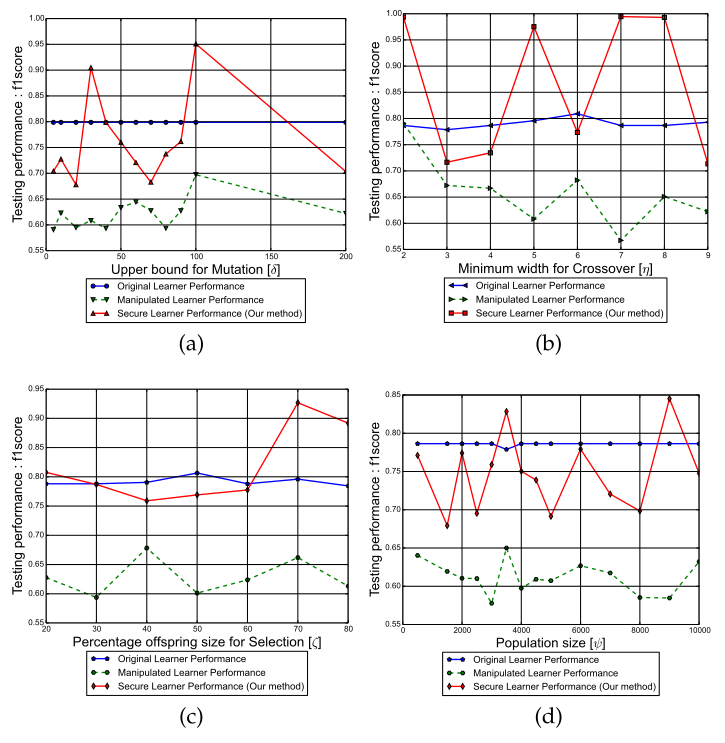
\includegraphics[scale=0.2]{images/Fig3abcd.png}
    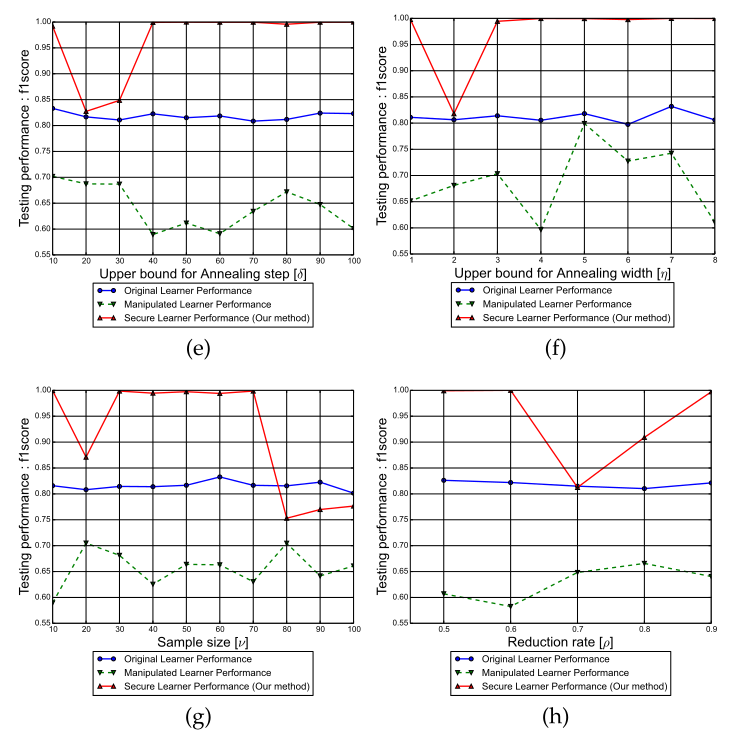
\includegraphics[scale=0.2]{images/Fig3defg.png}
    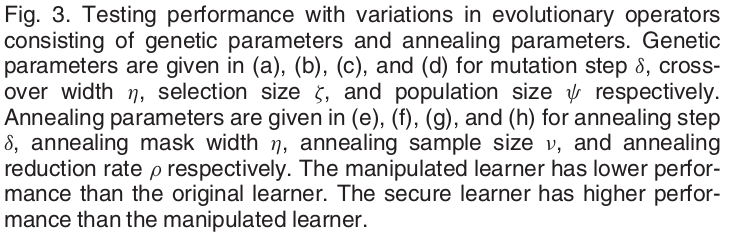
\includegraphics[width=8cm]{images/Fig3text.png}
\end{frame}

\begin{frame}{Testing Performance}
    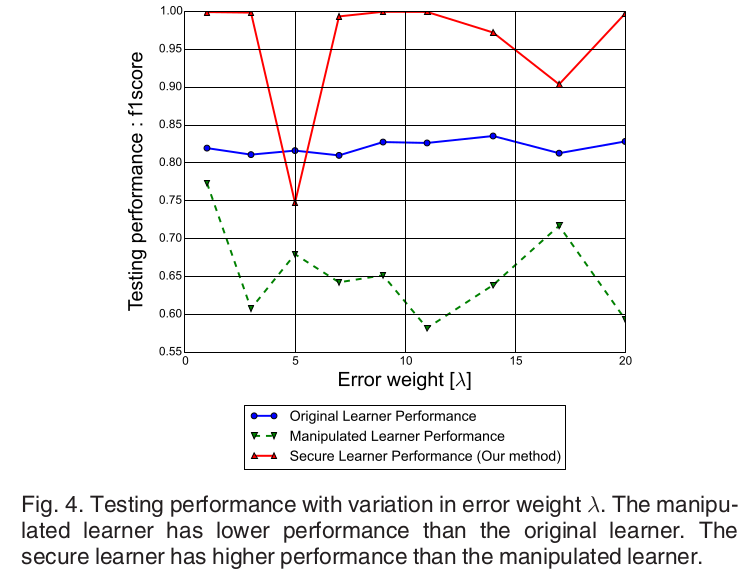
\includegraphics[scale=0.3]{images/Fig4.png}
\end{frame}


\begin{frame}{Observations}
	\begin{itemize}
        \item GA attacks are better than SA attacks, Multiplayer game attacks are better than two-player game attacks
        \item The t-statistics validate that our method is immune to various adversarial datasets.
        \item We demonstrate that the original CNN model as well as the GAN-based CNN model are vulnerable to proposed adversarial manipulations.
        \item Better search algorithms and optimization conditions would lead to adversarial data manipulations that are effective on both original data distributions as well as generated data distributions.
	\end{itemize}
\end{frame}





















% \subsection{Tricks}

% {
%     \metroset{titleformat frame=smallcaps}
% \begin{frame}{Small caps}
% 	This frame uses the \texttt{smallcaps} titleformat.

% 	\begin{alertblock}{Potential Problems}
% 		Be aware, that not every font supports small caps. If for example you typeset your presentation with pdfTeX and the Computer Modern Sans Serif font, every text in smallcaps will be typeset with the Computer Modern Serif font instead.
% 	\end{alertblock}
% \end{frame}
% }

% {
% \metroset{titleformat frame=allsmallcaps}
% \begin{frame}{All small caps}
% 	This frame uses the \texttt{allsmallcaps} titleformat.

% 	\begin{alertblock}{Potential problems}
% 		As this titleformat also uses smallcaps you face the same problems as with the \texttt{smallcaps} titleformat. Additionally this format can cause some other problems. Please refer to the documentation if you consider using it.

% 		As a rule of thumb: Just use it for plaintext-only titles.
% 	\end{alertblock}
% \end{frame}
% }

% {
% \metroset{titleformat frame=allcaps}
% \begin{frame}{All caps}
% 	This frame uses the \texttt{allcaps} titleformat.

% 	\begin{alertblock}{Potential Problems}
% 		This titleformat is not as problematic as the \texttt{allsmallcaps} format, but basically suffers from the same deficiencies. So please have a look at the documentation if you want to use it.
% 	\end{alertblock}
% \end{frame}
% }

% \section{Elements}

% \begin{frame}[fragile]{Typography}
%       \begin{verbatim}The theme provides sensible defaults to
% \emph{emphasize} text, \alert{accent} parts
% or show \textbf{bold} results.\end{verbatim}

%   \begin{center}becomes\end{center}

%   The theme provides sensible defaults to \emph{emphasize} text,
%   \alert{accent} parts or show \textbf{bold} results.
% \end{frame}

% \begin{frame}{Font feature test}
%   \begin{itemize}
%     \item Regular
%     \item \textit{Italic}
%     \item \textsc{SmallCaps}
%     \item \textbf{Bold}
%     \item \textbf{\textit{Bold Italic}}
%     \item \textbf{\textsc{Bold SmallCaps}}
%     \item \texttt{Monospace}
%     \item \texttt{\textit{Monospace Italic}}
%     \item \texttt{\textbf{Monospace Bold}}
%     \item \texttt{\textbf{\textit{Monospace Bold Italic}}}
%   \end{itemize}
% \end{frame}

% \begin{frame}{Lists}
%   \begin{columns}[T,onlytextwidth]
%     \column{0.33\textwidth}
%       Items
%       \begin{itemize}
%         \item Milk \item Eggs \item Potatos
%       \end{itemize}

%     \column{0.33\textwidth}
%       Enumerations
%       \begin{enumerate}
%         \item First, \item Second and \item Last.
%       \end{enumerate}

%     \column{0.33\textwidth}
%       Descriptions
%       \begin{description}
%         \item[PowerPoint] Meeh. \item[Beamer] Yeeeha.
%       \end{description}
%   \end{columns}
% \end{frame}
% \begin{frame}{Animation}
%   \begin{itemize}[<+- | alert@+>]
%     \item \alert<4>{This is\only<4>{ really} important}
%     \item Now this
%     \item And now this
%   \end{itemize}
% \end{frame}
% \begin{frame}{Figures}
%   \begin{figure}
%     \newcounter{density}
%     \setcounter{density}{20}
%     \begin{tikzpicture}
%       \def\couleur{alerted text.fg}
%       \path[coordinate] (0,0)  coordinate(A)
%                   ++( 90:5cm) coordinate(B)
%                   ++(0:5cm) coordinate(C)
%                   ++(-90:5cm) coordinate(D);
%       \draw[fill=\couleur!\thedensity] (A) -- (B) -- (C) --(D) -- cycle;
%       \foreach \x in {1,...,40}{%
%           \pgfmathsetcounter{density}{\thedensity+20}
%           \setcounter{density}{\thedensity}
%           \path[coordinate] coordinate(X) at (A){};
%           \path[coordinate] (A) -- (B) coordinate[pos=.10](A)
%                               -- (C) coordinate[pos=.10](B)
%                               -- (D) coordinate[pos=.10](C)
%                               -- (X) coordinate[pos=.10](D);
%           \draw[fill=\couleur!\thedensity] (A)--(B)--(C)-- (D) -- cycle;
%       }
%     \end{tikzpicture}
%     \caption{Rotated square from
%     \href{http://www.texample.net/tikz/examples/rotated-polygons/}{texample.net}.}
%   \end{figure}
% \end{frame}
% \begin{frame}{Tables}
%   \begin{table}
%     \caption{Largest cities in the world (source: Wikipedia)}
%     \begin{tabular}{lr}
%       \toprule
%       City & Population\\
%       \midrule
%       Mexico City & 20,116,842\\
%       Shanghai & 19,210,000\\
%       Peking & 15,796,450\\
%       Istanbul & 14,160,467\\
%       \bottomrule
%     \end{tabular}
%   \end{table}
% \end{frame}
% \begin{frame}{Blocks}
%   Three different block environments are pre-defined and may be styled with an
%   optional background color.

%   \begin{columns}[T,onlytextwidth]
%     \column{0.5\textwidth}
%       \begin{block}{Default}
%         Block content.
%       \end{block}

%       \begin{alertblock}{Alert}
%         Block content.
%       \end{alertblock}

%       \begin{exampleblock}{Example}
%         Block content.
%       \end{exampleblock}

%     \column{0.5\textwidth}

%       \metroset{block=fill}

%       \begin{block}{Default}
%         Block content.
%       \end{block}

%       \begin{alertblock}{Alert}
%         Block content.
%       \end{alertblock}

%       \begin{exampleblock}{Example}
%         Block content.
%       \end{exampleblock}

%   \end{columns}
% \end{frame}
% \begin{frame}{Math}
%   \begin{equation*}
%     e = \lim_{n\to \infty} \left(1 + \frac{1}{n}\right)^n
%   \end{equation*}
% \end{frame}
% \begin{frame}{Line plots}
%   \begin{figure}
%     \begin{tikzpicture}
%       \begin{axis}[
%         mlineplot,
%         width=0.9\textwidth,
%         height=6cm,
%       ]

%         \addplot {sin(deg(x))};
%         \addplot+[samples=100] {sin(deg(2*x))};

%       \end{axis}
%     \end{tikzpicture}
%   \end{figure}
% \end{frame}
% \begin{frame}{Bar charts}
%   \begin{figure}
%     \begin{tikzpicture}
%       \begin{axis}[
%         mbarplot,
%         xlabel={Foo},
%         ylabel={Bar},
%         width=0.9\textwidth,
%         height=6cm,
%       ]

%       \addplot plot coordinates {(1, 20) (2, 25) (3, 22.4) (4, 12.4)};
%       \addplot plot coordinates {(1, 18) (2, 24) (3, 23.5) (4, 13.2)};
%       \addplot plot coordinates {(1, 10) (2, 19) (3, 25) (4, 15.2)};

%       \legend{lorem, ipsum, dolor}

%       \end{axis}
%     \end{tikzpicture}
%   \end{figure}
% \end{frame}
% \begin{frame}{Quotes}
%   \begin{quote}
%     Veni, Vidi, Vici
%   \end{quote}
% \end{frame}

% {%
% \setbeamertemplate{frame footer}{My custom footer}
% \begin{frame}[fragile]{Frame footer}
%     \themename defines a custom beamer template to add a text to the footer. It can be set via
%     \begin{verbatim}\setbeamertemplate{frame footer}{My custom footer}\end{verbatim}
% \end{frame}
% }

% \begin{frame}{References}
%   Some references to showcase [allowframebreaks] \cite{knuth92,ConcreteMath,Simpson,Er01,greenwade93}
% \end{frame}

% \section{Conclusion}

% \begin{frame}{Summary}

%   Get the source of this theme and the demo presentation from

%   \begin{center}\url{github.com/matze/mtheme}\end{center}

%   The theme \emph{itself} is licensed under a
%   \href{http://creativecommons.org/licenses/by-sa/4.0/}{Creative Commons
%   Attribution-ShareAlike 4.0 International License}.

%   \begin{center}\ccbysa\end{center}

% \end{frame}

% {\setbeamercolor{palette primary}{fg=black, bg=yellow}
% \begin{frame}[standout]
%   Questions?
% \end{frame}
% }

% \appendix

% \begin{frame}[fragile]{Backup slides}
%   Sometimes, it is useful to add slides at the end of your presentation to
%   refer to during audience questions.

%   The best way to do this is to include the \verb|appendixnumberbeamer|
%   package in your preamble and call \verb|\appendix| before your backup slides.

%   \themename will automatically turn off slide numbering and progress bars for
%   slides in the appendix.
% \end{frame}

\begin{frame}[allowframebreaks]{References}

  \bibliography{demo}
  \bibliographystyle{abbrv}

\end{frame}

\end{document}
